\documentclass{beamer}

\usepackage{framed}
\usepackage{graphicx}

\begin{document}
\section{Statistical estimation within categories}

%====================================%
\begin{frame}[fragile]
	\frametitle{Seaborn Workshop}
	\large
\noindent \textbf{Statistical estimation within categories}
\begin{itemize}
\item Often, rather than showing the distribution within each category, you might want to show the central tendency of the values. 
\item Seaborn has two main ways to show this information, but importantly, the basic API for these functions is identical to that for the ones discussed above.
\end{itemize}
\end{frame}

%====================================%
\begin{frame}[fragile]
\frametitle{Seaborn Workshop}
\large
\noindent \textbf{Bar plots}
\begin{itemize}
\item A familiar style of plot that accomplishes this goal is a bar plot. 
\item In seaborn, the \texttt{barplot()} function operates on a full dataset and shows an arbitrary estimate, using the mean by default.
\item When there are multiple observations in each category, it also uses bootstrapping to compute a confidence interval around the estimate and plots that using error bars:
\end{itemize}

\end{frame}
%====================================%
\begin{frame}[fragile]

	\frametitle{Seaborn Workshop}
\large
\begin{verbatim}
sns.barplot(x="sex", y="survived", 
     hue="class", data=titanic);
\end{verbatim}
\begin{figure}
\centering
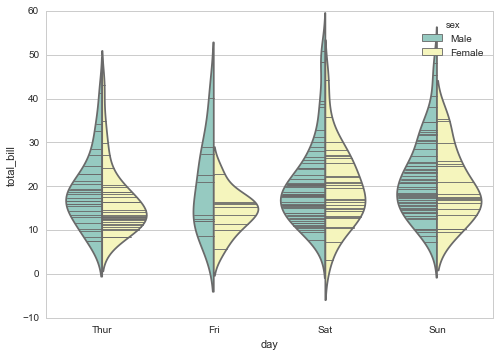
\includegraphics[width=0.9\linewidth]{images/categorical_29_0}
\end{figure}
\end{frame}
%====================================%
\begin{frame}[fragile]
	\frametitle{Seaborn Workshop}
	\large
\begin{itemize}
\item A special case for the bar plot is when you want to show the number of observations in each category rather than computing a statistic for a second variable. 
\item This is similar to a histogram over a categorical, rather than quantitative, variable. 
\item In seaborn, it’s easy to do so with the \texttt{countplot()} function:
\end{itemize}

\end{frame}
%====================================%
\begin{frame}[fragile]
	\frametitle{Seaborn Workshop}
	\large
	\begin{verbatim}
sns.countplot(x="deck", data=titanic, palette="Greens_d");
	\end{verbatim}

\begin{figure}
\centering
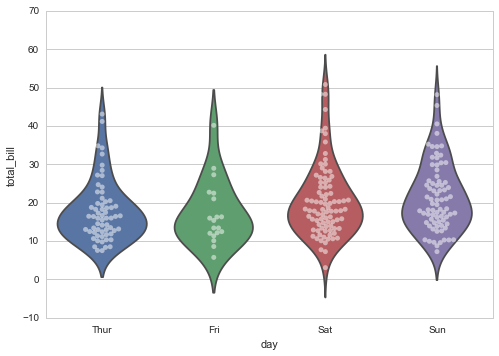
\includegraphics[width=0.7\linewidth]{images/categorical_31_0}
\end{figure}
\end{frame}
%======================================================================== %
\begin{frame}[fragile]
	\frametitle{Seaborn Workshop}
	\large
Both \texttt{barplot()} and \texttt{countplot()} can be invoked with all of the options discussed above, along with others that are demonstrated in the detailed documentation for each function:
\end{frame}
%======================================================================== %
\begin{frame}[fragile]
	\frametitle{Seaborn Workshop}
	\large
\begin{verbatim}
sns.countplot(y="deck", hue="class", 
     data=titanic, palette="Greens_d");
\end{verbatim}

\begin{figure}
\centering
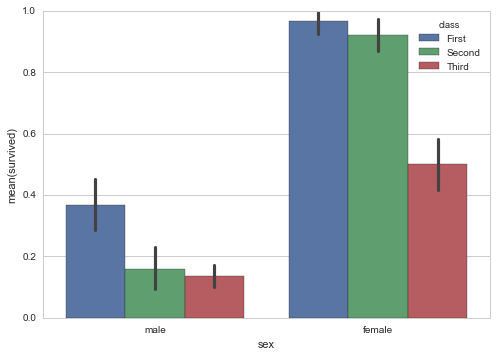
\includegraphics[width=0.75\linewidth]{images/categorical_33_0}
\end{figure}

\end{frame}
\section{Point plots}
%====================================%
\begin{frame}[fragile]
	\frametitle{Seaborn Workshop}
	\large
\noindent \textbf{Point plots}
\begin{itemize}
\item An alternative style for visualizing the same information is offered by the \texttt{pointplot()} function. 
\item This function also encodes the value of the estimate with height on the other axis, but rather than show a full bar it just plots the point estimate and confidence interval. 
\item Additionally, pointplot connects points from the same hue category. 
\item This makes it easy to see how the main relationship is changing as a function of a second variable, because your eyes are quite good at picking up on differences of slopes:
\end{itemize}

\end{frame}

%====================================%
\begin{frame}[fragile]
	\frametitle{Seaborn Workshop}
\large
\begin{verbatim}
sns.pointplot(x="sex", y="survived", hue="class", data=titanic);
\end{verbatim}
\begin{figure}
\centering
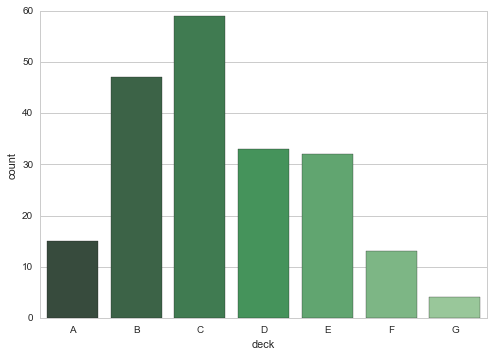
\includegraphics[width=0.7\linewidth]{images/categorical_35_0}
\end{figure}
\end{frame}
%================================================================================ %
\begin{frame}[fragile]
	\frametitle{Seaborn Workshop}
	\large
\begin{itemize}
\item To make figures that reproduce well in black and white, it can be good to use different markers and line styles for the levels of the hue category.
\end{itemize}
\begin{framed}
	\begin{verbatim}
	sns.pointplot(x="class", y="survived", 
	    hue="sex", data=titanic,
	    palette={"male": "g", "female": "m"},
	    markers=["^", "o"], 
	    linestyles=["-", "--"]);
	\end{verbatim}
\end{framed}
\end{frame}
%======================================================================== %
\begin{frame}[fragile]
	\frametitle{Seaborn Workshop}
	\large

\begin{figure}
\centering
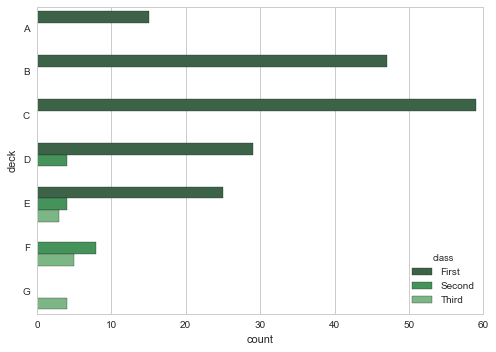
\includegraphics[width=0.9\linewidth]{images/categorical_37_0}
\end{figure}

\end{frame}
\end{document}

